% !TeX program = pdflatex
% !TeX spellcheck = de
% Copyright 2018-2022 FIUS
%
% This file is part of theo-vorkurs-folien.
%
% theo-vorkurs-folien is free software: you can redistribute it and/or modify
% it under the terms of the GNU General Public License as published by
% the Free Software Foundation, either version 3 of the License, or
% (at your option) any later version.
%
% theo-vorkurs-folien is distributed in the hope that it will be useful,
% but WITHOUT ANY WARRANTY; without even the implied warranty of
% MERCHANTABILITY or FITNESS FOR A PARTICULAR PURPOSE.  See the
% GNU General Public License for more details.
%
% You should have received a copy of the GNU General Public License
% along with theo-vorkurs-folien.  If not, see <https://www.gnu.org/licenses/>.

\documentclass[aspectratio=43,10pt]{beamer}

\usetheme[progressbar=frametitle]{metropolis}
\usepackage{appendixnumberbeamer}
\usepackage[ngerman]{babel}
\usepackage[utf8]{inputenc}
%\usepackage{t1enc}
\usepackage[T1]{fontenc}
\usepackage[sfdefault,scaled=.85,lf]{FiraSans}
\usepackage{newtxsf}

\usepackage{booktabs}
\usepackage[scale=2]{ccicons}
\usepackage{hyperref}

\usepackage{pgf}
\makeatletter
\@ifclasswith{beamer}{notes}{
  \usepackage{pgfpages}
  \setbeameroption{show notes on second screen}
}{}
\makeatother
\usepackage{tikz}
\usetikzlibrary{arrows,automata,positioning}
\usepackage{pgfplots}
\usepgfplotslibrary{dateplot}

\usepackage{xspace}
\newcommand{\themename}{\textbf{\textsc{metropolis}}\xspace}

\usepackage{blindtext}
\usepackage{graphicx}
\usepackage{subcaption}
\usepackage{comment}
\usepackage{mathtools}
\usepackage{amsmath}
\usepackage{centernot}
\usepackage{amssymb}
\usepackage{proof}
\usepackage{tabularx}
\renewcommand{\figurename}{Abb.}
\usepackage{marvosym}
\usepackage{mathtools}
\usepackage{qrcode}
\usepackage{advdate}

\newcommand\daynr{0}

\definecolor{ExColor}{HTML}{17819b}

\newcommand{\emptyWord}{\varepsilon}
\let \emptyset\varnothing
\newcommand{\SigmaStern}{\Sigma^{*}}
\newcommand{\absval}[1]{|#1|}
\newcommand{\defeq}{\vcentcolon=}
\newcommand{\eqdef}{=\vcentcolon}
\newcommand{\nimplies}{\centernot\implies}

\newcommand{\naturals}{\ensuremath{\mathbb{N}}}
\newcommand{\integers}{\ensuremath{\mathbb{Z}}}
\newcommand{\rationals}{\ensuremath{\mathbb{Q}}}
\newcommand{\reals}{\ensuremath{\mathbb{R}}}
\newcommand{\iffspace}{\ensuremath{\iff\;}}

\setbeamertemplate{footline}[text line]
{\parbox{\linewidth}{Fachgruppe Informatik\hfill\insertpagenumber\hfill Vorkurs Theoretische Informatik\vspace{0.2in}}}

\newcommand{\Center}[1]{
  \begin{frame}<handout:0>[standout]
    #1
  \end{frame}
}

% Fix section pages in appendix
\AtBeginDocument{%
  \apptocmd{\appendix}{%
    \setbeamertemplate{section page}[simple]%
  }{}{}
}

\addtobeamertemplate{block begin}{}{\vskip 0em}
\addtobeamertemplate{block alerted begin}{}{\vskip 0em}
\addtobeamertemplate{block example begin}{}{\vskip 0em}

% Copyright 2018-2022 FIUS
%
% This file is part of theo-vorkurs-folien.
%
% theo-vorkurs-folien is free software: you can redistribute it and/or modify
% it under the terms of the GNU General Public License as published by
% the Free Software Foundation, either version 3 of the License, or
% (at your option) any later version.
%
% theo-vorkurs-folien is distributed in the hope that it will be useful,
% but WITHOUT ANY WARRANTY; without even the implied warranty of
% MERCHANTABILITY or FITNESS FOR A PARTICULAR PURPOSE.  See the
% GNU General Public License for more details.
%
% You should have received a copy of the GNU General Public License
% along with theo-vorkurs-folien.  If not, see <https://www.gnu.org/licenses/>.



% Configuration for slides

% The date of the first day of the Theo-Vorkurs in Format dd/mm/yyyy
\SetDate[10/10/2022]

% Invite URL to the Ersti-Telegram-Group. Used for text on slide as well as QR-Code
\newcommand\telegramurl{https://t.me/+Q92w5biyY903NjEy}

% The url to the handout of the current day with the current day as argument. Used for the qr-code in the slides. 
\newcommand{\handouturl}[1]{https://fius.de/wp-content/uploads/2022/10/day-#1-handout.pdf}


\title{Vorkurs Theoretische Informatik}
\subtitle{Induktion und Einführung in die Grammatik}
\date{Mittwoch, 13.10.2021}
\author{Arbeitskreis Theo Vorkurs}
\institute{Fachgruppe Informatik}
% \titlegraphic{\hfill\includegraphics[height=1.5cm]{logo.pdf}}

\begin{document}

\maketitle

\begin{frame}[fragile]{Übersicht}
  \setbeamertemplate{section in toc}[sections numbered]
  \tableofcontents%[hideallsubsections]
\end{frame}

\section{Vollständige Induktion}

% Copyright 2018-2022 FIUS
%
% This file is part of theo-vorkurs-folien.
%
% theo-vorkurs-folien is free software: you can redistribute it and/or modify
% it under the terms of the GNU General Public License as published by
% the Free Software Foundation, either version 3 of the License, or
% (at your option) any later version.
%
% theo-vorkurs-folien is distributed in the hope that it will be useful,
% but WITHOUT ANY WARRANTY; without even the implied warranty of
% MERCHANTABILITY or FITNESS FOR A PARTICULAR PURPOSE.  See the
% GNU General Public License for more details.
%
% You should have received a copy of the GNU General Public License
% along with theo-vorkurs-folien.  If not, see <https://www.gnu.org/licenses/>.

\begin{frame}[fragile]{Idee}
    \begin{columns}
        \column{0.5\textwidth}
        \begin{alertblock}{Zeige Aussagen der Form:\\\emph{Für alle $n\in\mathbb{N}$ gilt\ldots}}
            \begin{enumerate}
                \item Zeige Aussage für das kleinste Element
                \item<1-> \only<7,8|handout:0>{\alert<7>{Zeige, wenn Aussage für beliebiges $n$ gilt, gilt sie auch für dessen Nachfolger, also $n+1$.}}\onslide<1-6>{Zeige, dass Aussage auch für das folgende Element gilt.}
                \item<2-6,8> \only<8|handout:0>{\alert<8>{$\leadsto$ Aussage gilt für alle $n$.}}\onslide<2-6>{\small Zeige, dass Aussage auch für das folgende Element gilt.}
                \item<3-6> \footnotesize Zeige, dass Aussage auch für das folgende Element gilt.
                \item<4-6> \scriptsize Zeige, dass Aussage auch für das folgende Element gilt.
                \item<5-6> \tiny Zeige, dass Aussage auch für das folgende Element gilt.
                \item<6> \dots
            \end{enumerate}
        \end{alertblock}
        \column{0.5\textwidth}
        \begin{figure}
            \centering
            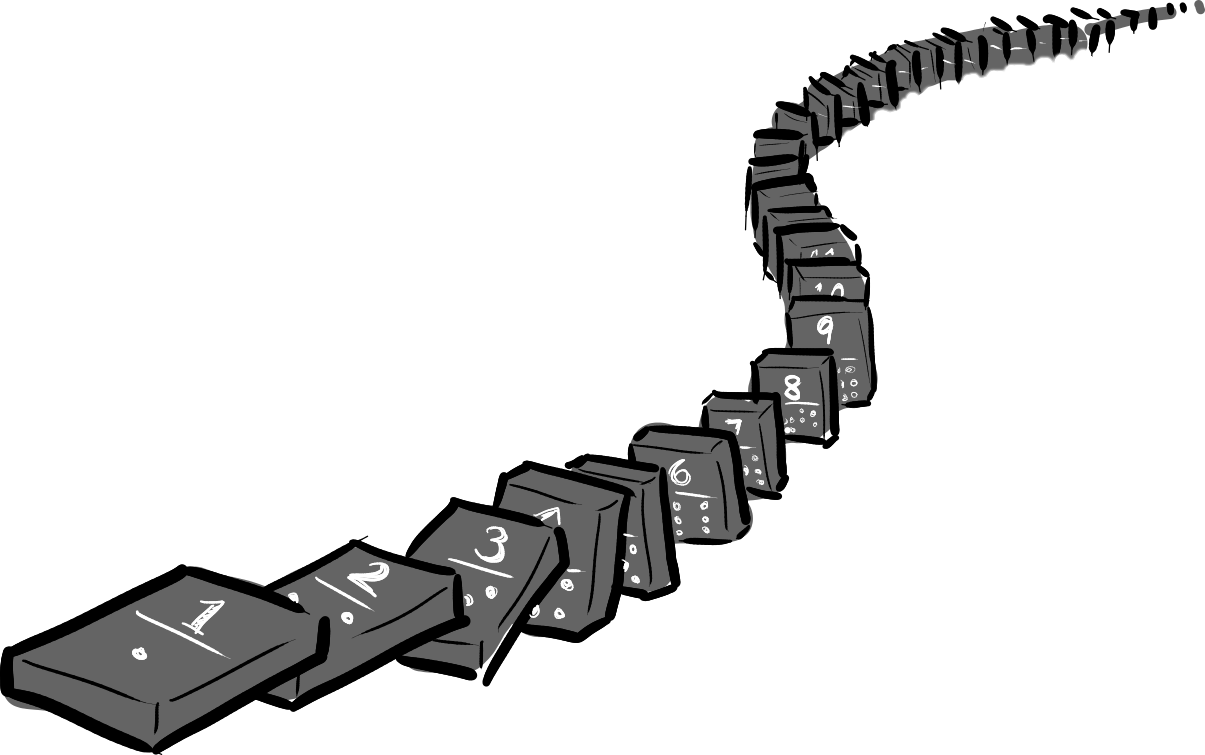
\includegraphics[width=0.7\textwidth]{../figures/induction.png}
            %\caption{Idee}
            %
        \end{figure}
    \end{columns}
\end{frame}

\subsection{Funktionsweise}
\begin{frame}[fragile]{Struktur}
    \begin{alertblock}{Zeige Aussagen der Form:\\\emph{Für alle $n\in\mathbb{N}$ gilt\ldots}}
        \begin{enumerate}
            \item \alert{Induktionsanfang}\\Zeige Aussage für das kleinste Element
            \item \alert{Induktionsvoraussetzung}\\Zeige, unter der Voraussetzung: \\\emph{die Aussage gelte für beliebiges $n$},\dots
            \item \alert{Induktionsschritt}\\\dots dann gilt die Aussage auch für dessen Nachfolger $n+1$.
            \item $\leadsto$ Aussage gilt für alle $n \in \mathbb{N}$.
        \end{enumerate}
    \end{alertblock}
\end{frame}

\begin{frame}[fragile]{Beispiel}
    \center $\displaystyle\sum_{i = 0}^{n} (2i+1) = (n+1)^2,\quad\forall n \in\mathbb{N}$.
    \begin{figure}
        \centering
        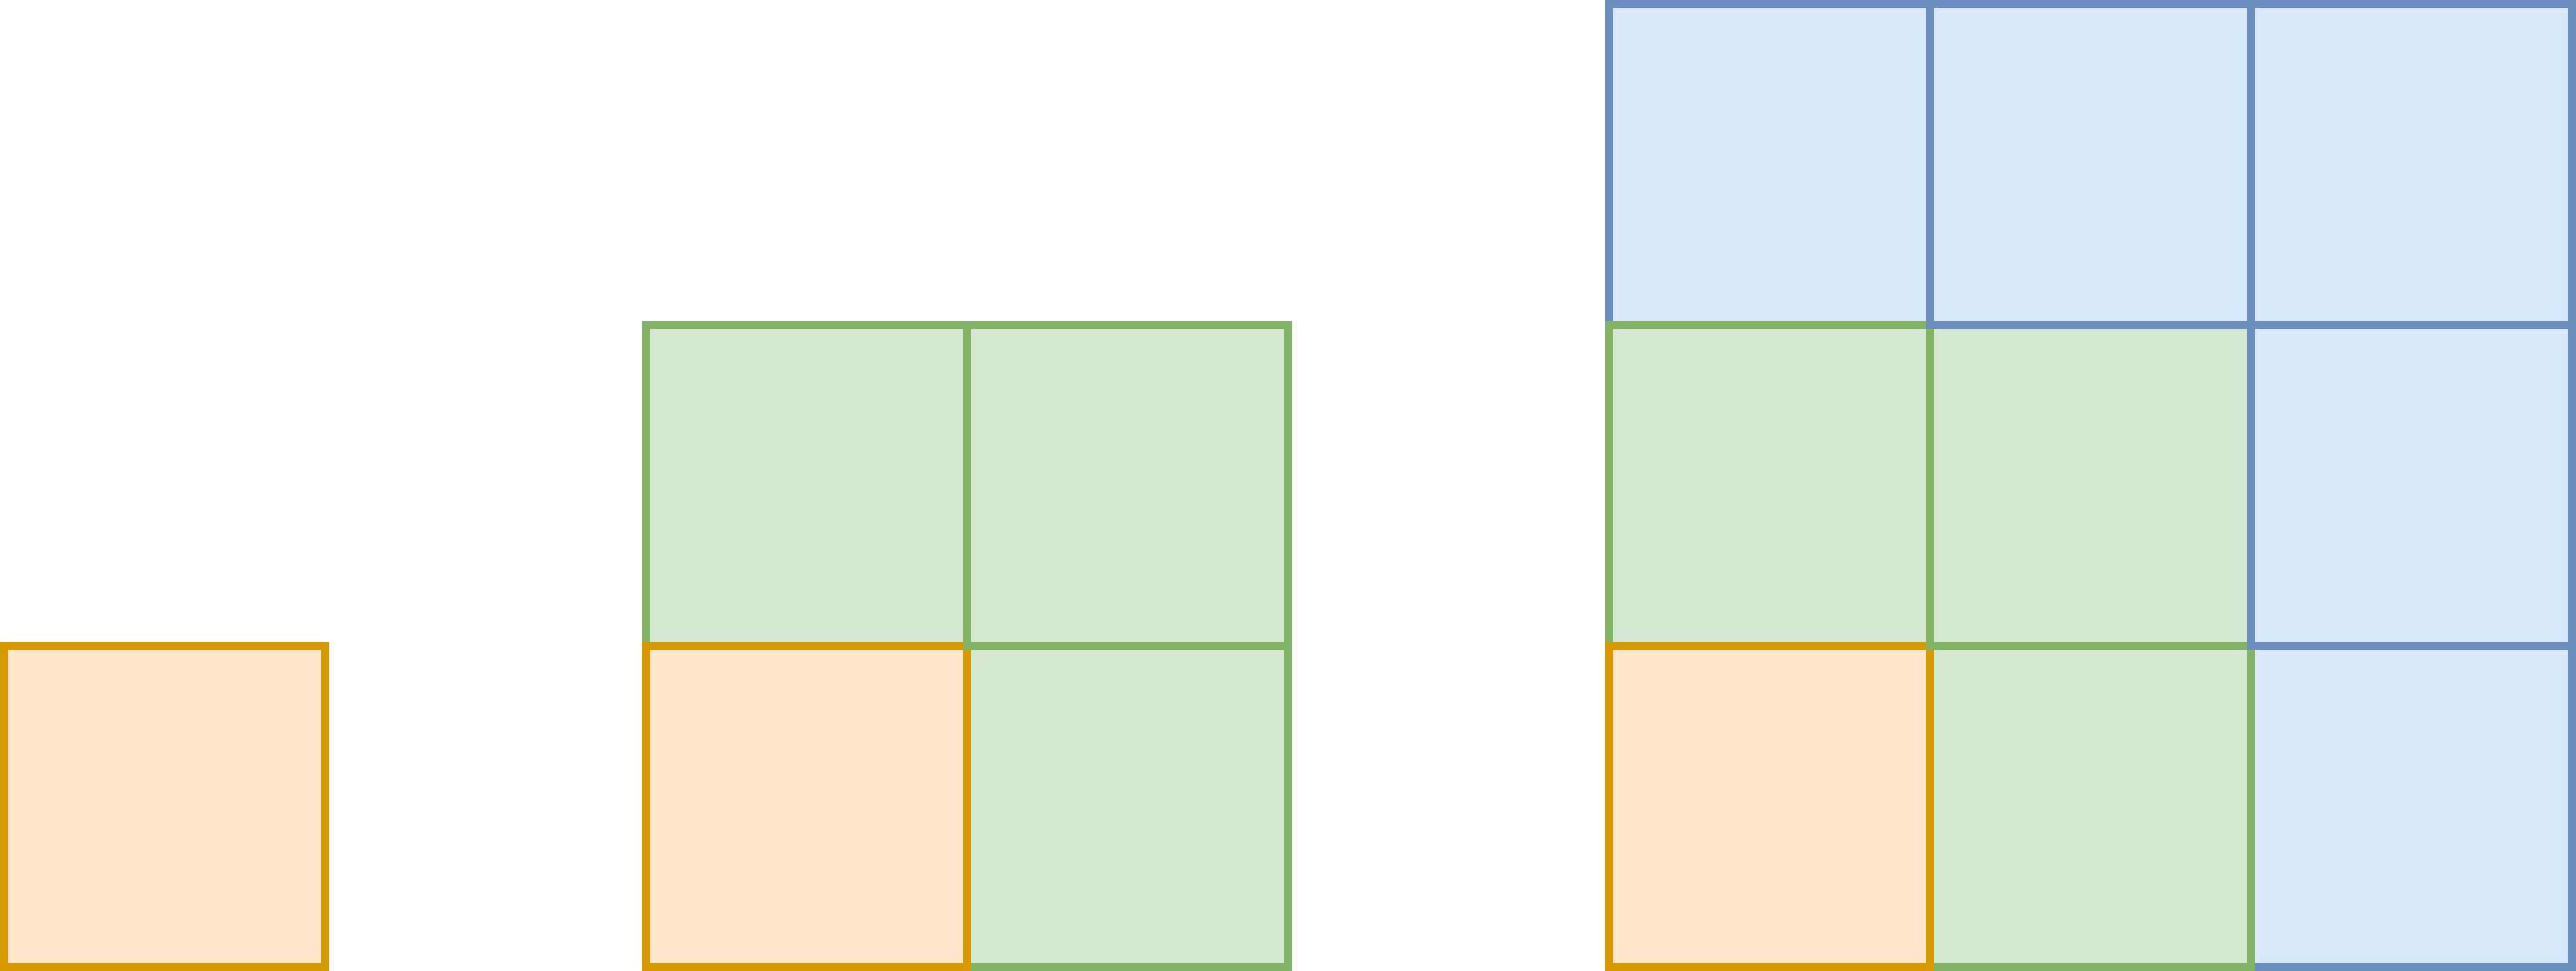
\includegraphics[width=0.5\textheight]{../figures/Summe.png}\qquad \dots
        %\caption{Idee}
        %
    \end{figure}
\end{frame}
\note[itemize]{
    \item Idee: Es werden 1, 3, 5, \ldots Felder hinzugenommen
    \item Lässt sich jeweils zu einem Quadrat zusammensetzen
    \item Mit jedem Schritt wird Kantenlänge des Quadrats um eins größer
}

\begin{frame}[fragile]{Beispiel}
    Zeigen Sie $\displaystyle\sum_{i = 0}^{n} (2i+1) = (n+1)^2,\quad\forall n \in\mathbb{N}$.
    \begin{alertblock}{Induktionsanfang (IA)}
        Zeige Aussage gilt für $n\defeq0$:\\
        \begin{align*}
                      & \sum_{i = 0}^{0} (2i+1) &  & \overset{!}{=} &  & (0+1)^2 &                  \\
            \iffspace & 2 \cdot 0 + 1           &  & \overset{!}{=} &  & 1^2     &                  \\
            \iffspace & 1                       &  & =              &  & 1       & \qquad\checkmark
        \end{align*}
    \end{alertblock}
\end{frame}

\begin{frame}[fragile]{Beispiel}
    Zeigen Sie $\displaystyle\sum_{i = 0}^{n} (2i+1) = (n+1)^2,\quad\forall n \in\mathbb{N}$.
    \begin{alertblock}{Induktionsanfang (IA)}
        Aussage gilt für $n\defeq0$, da $\displaystyle\sum_{i = 0}^{0} (2i+1) = (0+1)^2$.
    \end{alertblock}
    \begin{alertblock}{Induktionsvoraussetzung (IV)}
        Ang. Aussage gilt für (ein beliebiges aber festes) $n \in\mathbb{N}$.
    \end{alertblock}
    \begin{alertblock}{Induktionsschritt (IS)}
        Zeige Aussage gilt für alle $n+1$ unter Nutzung der (IV):\par
        $\displaystyle\sum_{i = 0}^{\alert{n+1}} (2i+1) \overset{!}{=} (\alert{(n+1)}+1)^2$
    \end{alertblock}
\end{frame}

\begin{frame}[fragile]{Beispiel}
    \small\begin{alertblock}{Induktionsschritt}
        Zeige Aussage gilt für alle $n+1$ unter Nutzung der IV:\@
        \begin{align*}
            \onslide<1->{                                 & \sum_{i = 0}^{n+1} (2i+1)                                                   &  & \overset{!}{=} &  & ((n+1)+1)^2            & } \\
            \onslide<2->{\iffspace                        & \sum_{i = 0}^{\alert<2>{n}} (2i+1) + \sum_{i = \alert<2>{n+1}}^{n+1} (2i+1) &  & \overset{!}{=} &  & (n+2)^2                & } \\
            \onslide<3->{\iffspace                        & \sum_{i = 0}^{n} (2i+1) + ( 2(n+1)+1 )                                      &  & \overset{!}{=} &  & n^2 + 2 \cdot 2n + 2^2 & } \\
            \onslide<4->{\overset{\alert<4>{IV}}\iffspace & \alert<4>{(n+1)^2} + ( 2(n+1)+1 )                                           &  & \overset{!}{=} &  & n^2+4n+4               & } \\
            \onslide<5->{\iffspace                        & n^2+2n+1^2+2n+2+1                                                           &  & \overset{!}{=} &  & n^2+4n+4               & } \\
            \onslide<6>{\iffspace                         & n^2+4n+4                                                                    &  & \alert<6>{=}   &  & n^2+4n+4               & }
        \end{align*}
    \end{alertblock}
\end{frame}

\begin{frame}[fragile]{Beispiel}
    Zeigen Sie $\displaystyle\sum_{i = 0}^{n} (2i+1) = (n+1)^2, \quad\forall n \in\mathbb{N}$.
    \begin{alertblock}{Induktionsanfang (IA)}
        Aussage gilt für $n\defeq0$, da $\displaystyle\sum_{i = 0}^{0} (2i+1) = 1^2$.
    \end{alertblock}
    \begin{alertblock}{Induktionsvoraussetzung (IV)}
        Ang. Aussage gilt für (ein beliebiges aber festes) $n \in\mathbb{N}$.
    \end{alertblock}
    \begin{alertblock}{Induktionsschritt (IS)}
        Aussage gilt für alle $n+1$ unter Nutzung der IV, da\par
        $\displaystyle\sum_{i = 0}^{n+1} (2i+1) = ((n+1)+1)^2$
    \end{alertblock}
    \alert{$\leadsto$ Aussage gilt für alle n.}\qed
\end{frame}


{\setbeamercolor{palette primary}{bg=ExColor}
\begin{frame}[fragile]{Denkpause}
    \begin{alertblock}{Aufgaben}
        Versuche dich an den folgenden Induktionsbeweisen.
    \end{alertblock}

    \metroset{block=fill}
    \begin{block}{Normal}
        $\displaystyle\sum_{i=0}^{n} i = \frac{n(n+1)}{2}, \quad \forall n \in \mathbb{N}$
    \end{block}
    \begin{block}{Schwerer}
        $\displaystyle\prod_{i=1}^{n} 4^i = 2^{n(n+1)}, \quad \forall n \in \mathbb{N}\setminus \{0\}$
    \end{block}
\end{frame}
}

%\subsubsection{Lösungen normal}
{\setbeamercolor{palette primary}{bg=ExColor}
\begin{frame}<handout:0>[fragile]{Lösungen: normale Aufgabe}
    Zu zeigen: $\displaystyle\sum_{i=0}^{n} i = \frac{n(n+1)}{2}$ gilt für alle $n \in \mathbb{N}$.
    \begin{alertblock}{Induktionsanfang (IA)}
        Aussage gilt für $n\defeq 0$, da $\displaystyle\sum_{i=0}^{0} i = 0 = \frac{0(0+1)}{2}$.
    \end{alertblock}
    \begin{alertblock}{Induktionsvoraussetzung (IV)}
        Ang. Aussage gilt für $n \in\mathbb{N}$.
    \end{alertblock}
    \begin{alertblock}{Induktionsschritt (IS)}
        Zeige Aussage gilt für alle $n+1$ unter Nutzung der IV:\par
        $\displaystyle\sum_{i=0}^{\alert{n+1}} i \overset{!}{=} \frac{(\alert{n+1})\left((\alert{n+1})+1\right)}{2}$
    \end{alertblock}
\end{frame}


\begin{frame}<handout:0>[fragile]{Lösungen: normale Aufgabe}
    \small\begin{alertblock}{Induktionsschritt}
        Zeige Aussage gilt für $n+1$ unter Nutzung der I.V.:
        \begin{align*}
            \onslide<1->{                                 & \displaystyle\sum_{i=0}^{\alert<1>{n+1}} i       &  & \overset{!}{=} &  & \frac{(\alert<1>{n+1})\left((\alert<1>{n+1})+1\right)}{2} & } \\
            \onslide<2->{\iffspace                        & \left(\displaystyle\sum_{i=0}^{n} i\right)+(n+1) &  & \overset{!}{=} &  & \frac{(n+1)(n+2)}{2}                                      & } \\
            \onslide<3->{\iffspace                        & \left(\displaystyle\sum_{i=0}^{n} i\right)+(n+1) &  & \overset{!}{=} &  & \frac{n^2+3n+2}{2}                                        & } \\
            \onslide<4->{\overset{\alert<4>{IV}}\iffspace & \alert<4>{\frac{n(n+1)}{2}}+(n+1)                &  & \overset{!}{=} &  & \frac{n^2+3n+2}{2}                                        & } \\
            \onslide<5->{\iffspace                        & \frac{n^2+n}{2}+\frac{2n+2}{2}                   &  & \overset{!}{=} &  & \frac{n^2+3n+2}{2}                                        & } \\
            \onslide<6->{\iffspace                        & \frac{n^2+3n+2}{2}                               &  & \alert{=}      &  & \frac{n^2+3n+2}{2}                                        & } \\
        \end{align*}
    \end{alertblock}
\end{frame}


\begin{frame}<handout:0>[fragile]{Lösungen: normale Aufgabe}
    Zu zeigen: $\displaystyle\sum_{i=0}^{n} i = \frac{n(n+1)}{2}$ gilt für alle $n \in \mathbb{N}$.
    \begin{alertblock}{Induktionsanfang (IA)}
        Aussage gilt für $n\defeq 0$, da $\displaystyle\sum_{i=0}^{0} i = 0 = \frac{0(0+1)}{2}$.
    \end{alertblock}
    \begin{alertblock}{Induktionsvoraussetzung (IV)}
        Ang. Aussage gilt für $n \in\mathbb{N}$.
    \end{alertblock}
    \begin{alertblock}{Induktionsschritt (IS)}
        Zeige Aussage gilt für $n+1$ unter Nutzung der IV:\par
        $\displaystyle\sum_{i=0}^{\alert{n+1}} i \overset{!}{=} \frac{(\alert{n+1})\left((\alert{n+1})+1\right)}{2}$ gilt für alle $n \in \mathbb{N}$
    \end{alertblock}
    \alert{$\leadsto$ Aussage gilt für alle $n$.}\qed
\end{frame}
}

% \begin{frame}[standout]
%   Fragen dazu?
% \end{frame}

%\subsubsection{Lösungen schwerer}
{\setbeamercolor{palette primary}{bg=ExColor}
\begin{frame}<handout:0>[fragile]{Lösungen: schwerere Aufgabe}
    Zu zeigen: $\displaystyle\prod_{i=1}^{n} 4^i = 2^{n(n+1)}$ gilt für alle $n \in \mathbb{N}\setminus \{0\}$.
    \begin{alertblock}{Induktionsanfang (IA)}
        Aussage gilt für $n\defeq 1$, da $\displaystyle\prod_{i=1}^{1} 4^i = 4^1 = 4 = 2^2 = 2^{1(1+1)}$.
    \end{alertblock}
    \begin{alertblock}{Induktionsvoraussetzung (IV)}
        Ang. Aussage gilt für $n \in\mathbb{N}\setminus \{0\}$.
    \end{alertblock}
    \begin{alertblock}{Induktionsschritt (IS)}
        Zeige Aussage gilt für $n+1$ unter Nutzung der IV:\par
        $\displaystyle\prod_{i=1}^{\alert{n+1}} 4^i \overset{!}{=} 2^{(\alert{n+1})((\alert{n+1})+1)}$
    \end{alertblock}
\end{frame}

\begin{frame}<handout:0>[fragile]{Lösungen: schwerere Aufgabe}
    \small\begin{alertblock}{Induktionsschritt}
        Zeige Aussage gilt für $n+1$ unter Nutzung der I.V.:
        \begin{align*}
            \onslide<1->{                                 & \displaystyle\prod_{i=1}^{\alert<1>{n+1}} 4^i                 &  & \overset{!}{=} &  & 2^{(\alert<1>{n+1})((\alert<1>{n+1})+1)} & } \\
            \onslide<2->{\iffspace                        & \left(\displaystyle\prod_{i=1}^{n} 4^i\right) \cdot 4^{(n+1)} &  & \overset{!}{=} &  & 2^{(n+1)(n+2)}                           & } \\
            \onslide<3->{\overset{\alert<3>{IV}}\iffspace & \alert<3>{\left(2^{n(n+1)}\right)} \cdot 4^{(n+1)}            &  & \overset{!}{=} &  & 2^{n^2+3n+2}                             & } \\
            \onslide<4->{\iffspace                        & 2^{n^2+n} \cdot 2^{2(n+1)}                                    &  & \overset{!}{=} &  & 2^{n^2+3n+2}                             & } \\
            \onslide<5->{\iffspace                        & 2^{n^2+n} \cdot 2^{2n+2}                                      &  & \overset{!}{=} &  & 2^{n^2+3n+2}                             & } \\
            \onslide<6->{\iffspace                        & 2^{(n^2+n)+(2n+2)}                                            &  & \overset{!}{=} &  & 2^{n^2+3n+2}                             & } \\
            \onslide<7->{\iffspace                        & 2^{n^2+3n+2}                                                  &  & \alert{=}      &  & 2^{n^2+3n+2}                             & }
        \end{align*}
    \end{alertblock}
\end{frame}


\begin{frame}<handout:0>[fragile]{Lösungen: schwerere Aufgabe}
    Zu zeigen: $\displaystyle\prod_{i=1}^{n} 4^i = 2^{n(n+1)}$ gilt für alle $n \in \mathbb{N}\setminus \{0\}$.
    \begin{alertblock}{Induktionsanfang (IA)}
        Aussage gilt für $n\defeq 1$, da $\displaystyle\prod_{i=1}^{1} 4^i = 4^1 = 4 = 2^2 = 2^{1(1+1)}$.
    \end{alertblock}
    \begin{alertblock}{Induktionsvoraussetzung (IV)}
        Ang. Aussage gilt für $n \in\mathbb{N}\setminus \{0\}$.
    \end{alertblock}
    \begin{alertblock}{Induktionsschritt (IS)}
        Zeige Aussage gilt für $n+1$ unter Nutzung der IV:\par
        $\displaystyle\prod_{i=1}^{\alert{n+1}} 4^i \overset{!}{=} 2^{(\alert{n+1})((\alert{n+1})+1)}$ gilt für alle $n \in \mathbb{N}\setminus \{0\}$
    \end{alertblock}
    \alert{$\leadsto$ Aussage gilt für alle $n$.}\qed
\end{frame}
}

% \begin{frame}[standout]
%   Fragen dazu?
% \end{frame}


\begin{frame}<handout:0>[standout]
  Murmelpause
\end{frame}

% Copyright 2018-2022 FIUS
%
% This file is part of theo-vorkurs-folien.
%
% theo-vorkurs-folien is free software: you can redistribute it and/or modify
% it under the terms of the GNU General Public License as published by
% the Free Software Foundation, either version 3 of the License, or
% (at your option) any later version.
%
% theo-vorkurs-folien is distributed in the hope that it will be useful,
% but WITHOUT ANY WARRANTY; without even the implied warranty of
% MERCHANTABILITY or FITNESS FOR A PARTICULAR PURPOSE.  See the
% GNU General Public License for more details.
%
% You should have received a copy of the GNU General Public License
% along with theo-vorkurs-folien.  If not, see <https://www.gnu.org/licenses/>.

%Vollständige Induktion aus Tag 2
% \section{Wiederholung: Vollständige Induktion}

% \subsection{Definition}

% \begin{frame}[fragile]{Definition}
%  \begin{enumerate}
%      \item \textbf{Induktionsanfang} (Gilt die Aussage für ein $n_0$) \\
%      \item \textbf{Induktionsvoraussetzung} (wir nehmen dann an, die Aussage gilt tatsächlich)
%      \item \textbf{Induktionsschritt} (Hier zeigen wir, dass für alle $n \in \mathbb{N}$ die Aussage gilt, unter Verwendung der IV)
%  \end{enumerate}
% \end{frame}

\subsubsection{formalere Definition}
\begin{frame}{Definition nochmal formaler}
    \begin{equation*}
        (\forall n \in \mathbb{N}_{n_0}: P(n)) \iff (P(n_0) \wedge \forall n \in \mathbb{N}_{n_0}: (P(n) \implies P(n+1)))
    \end{equation*}    
\end{frame}

\begin{frame}{Definition nochmal formaler}
    \onslide<1->$(\forall n \in \mathbb{N}_{n_0}: P(n)) \iff (\alert<2>{\underbrace{P(n_0)}_{\text{IA}}}\wedge \overbrace{\alert<3>{\forall n \in \mathbb{N}_{n_0}:} (\alert<4>{\underbrace{P(n)}_{\text{IV}}} \alert<5>{\implies P(n+1)})}^{\text{IS}})$
    \begin{enumerate}
        \item<2->\alert<2>{\textbf{IA:} $n = n_0$}
        \item<3->\onslide<3->{\alert<3>{\textbf{IS:} Sei $n\in\mathbb{N}_{n_0}$ beliebig.}}
        \onslide<4->{\alert<4>{Ang. es gilt $P(n)$. \tiny{\textbf{(IV)}}}}    
        \item<5->\alert{$\leadsto$ Zeigen, dass $P(n+1)$ gilt, unter Verwendung von $P(n)$ \tiny{\textbf{(IV)}}}
    \end{enumerate}
\end{frame}

% \begin{frame}{Aufgabe zur Wiederholung}
%  Warum das ganze nur für Summen.\\
%  Angenommen $n^3-n$ ist durch 3 teilbar für alle natürlichen Zahlen.\\
%  Wie gehen wir dann hier vor?
% \end{frame}

% \begin{frame}{Aufgabe zur Wiederholung}
%  \begin{itemize}
%      \item<1->
%          Schreiben wir das ganze erst mal etwas Mathematischer.
%      \item<2->
%          $3 \mid n^3-n$, also 3 teilt $n^3-n$
%      \item<3->
%          Jetzt vollständige Induktion
%  \end{itemize}
% \end{frame}

% \begin{frame}{Vollständige Induktion}
%  \begin{enumerate}
%      \item<1->
%          \textbf{IA:} n = 1
%              \begin{equation*}
%                  3 \mid 1^3 - 1 \iff 3 \mid 1 - 1 \iff 3 \mid 0 \qquad \checkmark
%              \end{equation*}
%      \item<2->
%          % \textbf{IV:}\\
%          % Da $3 \mid n^3-n$ für 1 gilt, existiert also eine Zahl $n\in \mathbb{N}$ (beliebig aus den natürlichen Zahlen, hier 1 da wir es bereits dafür gezeigt haben), für welche die Aussage $3 \mid n^3 -n$ gilt.
%           \textbf{IS:} Sei $n \in \mathbb{N}$ beliebig. Ang., es gilt $3\mid n^3-n$ (IV)
%          \begin{align*}
%              3 \mid (n+1)^3-(n+1) &\iff 3\mid(n+1)^3 - n - 1\\
%              &\iff 3\mid n^3 + 3n^2 + 3n + 1 - n - 1\\
%              &\iff 3\mid \underbrace{n^3 - n}_{\text{Induktionsvoraussetzung}} + \underbrace{3n^2 + 3n}_{\text{vielfache von 3}} + \underbrace{1 - 1}_{= 0}\\
%              &\iff 3\mid(n^3 - n) + 3(n^2 + n)
%          \end{align*}
%      \item<3->
%      \textbf{Fazit:}\\
%          Nach Voraussetzung ist der erste Summand durch 3 teilbar, und der zweite Summand ist ein vielfaches von 3. Somit ist auch die Summe durch 3 teilbar.
%  \end{enumerate}
% \end{frame}

% \begin{frame}[fragile]{Ein Aufgabe zur Übung}
%  \begin{itemize}
%      \item Zeigen Sie, dass für alle natürlichen Zahlen $n \geq 4$ gilt: \\
%      \begin{center}
%          $n! > 2^n$\\
%      \end{center}
%  \end{itemize}
% \end{frame}

% {\setbeamercolor{palette primary}{bg=ExColor}
% \begin{frame}{Lösung}
%  \begin{enumerate}
%      \item
%          \textbf{IA:} n = 4
%          \begin{equation*}
%              4! = 4 \cdot 3 \cdot 2 \cdot 1 = 24 > 16 = 2^4
%          \end{equation*}
%      \item
%          \textbf{IV:}
%          Die Aussage $n! > 2^n$ gilt für n=4, also existiert ein $x\in \mathbb{N}$, sodass diese Aussage gilt.
%      \item
%          \textbf{IS:} Also gilt die Aussage für n+1
%          \begin{align*}
%              (n+1)! &= (n+1) \cdot n!\\
%              &\overset{\text{nach IV.}}{>} \underbrace{(n+1)}_{\text{da n min. 4}} \cdot 2^n\\
%              &\overset{(n+1)>2}{>} 2 \cdot 2^n = 2^{n+1}
%          \end{align*}
%      \item
%          \textbf{Fazit:}\\
%          Somit ist für alle $n\in \mathbb{N}$(beliebige natürliche Zahl) gezeigt, dass $n! > 2^n$ für $n \geq 4$.
%  \end{enumerate}
% \end{frame}
% }

% %An der Tafel die Lösung besprechen 


% Copyright 2018-2022 FIUS
%
% This file is part of theo-vorkurs-folien.
%
% theo-vorkurs-folien is free software: you can redistribute it and/or modify
% it under the terms of the GNU General Public License as published by
% the Free Software Foundation, either version 3 of the License, or
% (at your option) any later version.
%
% theo-vorkurs-folien is distributed in the hope that it will be useful,
% but WITHOUT ANY WARRANTY; without even the implied warranty of
% MERCHANTABILITY or FITNESS FOR A PARTICULAR PURPOSE.  See the
% GNU General Public License for more details.
%
% You should have received a copy of the GNU General Public License
% along with theo-vorkurs-folien.  If not, see <https://www.gnu.org/licenses/>.

{\setbeamercolor{palette primary}{bg=ExColor}
	\begin{frame}[fragile]{Aufgabe}
		\metroset{block=fill}
		\begin{alertblock}{Die folgende Induktion zeigt eine seltsame Aussage.}
			Ist der Beweis korrekt geführt? Was ist passiert?
		\end{alertblock}
		\metroset{block=transparent}
		Sei $A(n)\defeq$ \emph{In einer Herde aus $n$ Telefonen haben alle die selbe Farbe.}\\
		Zu zeigen: $A(n)$ gilt für alle $n \in \mathbb{N} \setminus \{0\} $.
		\begin{alertblock}{Induktionsanfang (IA)}
			$A(1)$: Aussage gilt für $n\defeq 1$, da ein Telefon nur eine Farbe haben kann.
		\end{alertblock}
		\begin{alertblock}{Induktionsvoraussetzung (IV)}
			Ang. $A(n)$ gilt für $n\geq1$.
		\end{alertblock}
		\begin{alertblock}{Induktionsschritt (IS)}
			Zeige Aussage gilt für alle $n+1$ unter Nutzung der IV:\\
			D.h. wir zeigen $A(n+1)=$ \emph{In einer Herde aus $n+1$ Telefonen haben alle die selbe Farbe.}
		\end{alertblock}
	\end{frame}
	\begin{frame}[fragile]{Aufgabe}
		\footnotesize{
			\begin{alertblock}{Induktionsschritt (IS)}
				Wir betrachten eine Herde aus $n+1$ Telefonen:
				\[\underbrace{\text{\Telefon}\text{\Telefon}\text{\Telefon}\text{\Telefon}\text{\Telefon}\dots\text{\Telefon}\text{\Telefon}}_{n+1}\]
				Wir sondern ein Telefon aus und betrachten den Rest. Nach I.V. haben diese alle die selbe Farbe.
				\[\underbrace{\alert{\text{\Telefon}\text{\Telefon}\text{\Telefon}\text{\Telefon}\text{\Telefon}\dots\text{\Telefon}}}_{n}\text{\Telefon}\]
				Jetzt sondern wir ein anderes Telefon aus.
				\[\alert{\text{\Telefon}}\underbrace{\alert{\text{\Telefon}\text{\Telefon}\text{\Telefon}\text{\Telefon}\dots\text{\Telefon}}\text{\Telefon}}_{n}\]
				Die übrigen $n$ Telefone haben nach I.V. wieder die selbe Farbe.
				\[\underbrace{\alert{\text{\Telefon}\text{\Telefon}\text{\Telefon}\text{\Telefon}\text{\Telefon}\dots\text{\Telefon}\text{\Telefon}}}_{n+1}\]
				Also haben alle $n+1$ Telefone die selbe Farbe.
				$\leadsto$ $A(n)$ gilt für alle $n$.
			\end{alertblock}
		}
	\end{frame}
}

{\setbeamercolor{palette primary}{bg=ExColor}
	\begin{frame}<handout:0>[fragile]{Lösungen}
		\small{
			\metroset{block=fill}
			\begin{block}{Das Problem}
				Für $A(n+1)$ wird angenommen, dass beide Herden der $n$ Telefone mindestens ein gemeinsames Element haben. 
				Sie teilen dann die Farbe dieses Elements. 

				Das Problem ist, dass $A(1) \Rightarrow A(2)$ nicht zwangsweise erfüllt sein muss! Somit können wir keine weiteren Folgerungen über $A(n+1)$ mit $n \geq 2$ machen.
				
				\begin{figure}
				\resizebox{.4\textwidth}{!}{
					\centering%
					\begin{subfigure}{0.3\textwidth}
						\centering%
						
\includegraphics[height=0.5in]{../figures/telephoneGreen.png}
					\end{subfigure}
					$\qquad$
					\begin{subfigure}{0.3\textwidth}
						\centering%
						
\includegraphics[height=0.5in]{../figures/telephoneWhite.png}
					\end{subfigure}
					}
					\caption{Beide Telefone erfüllen jeweils $A(1)$, zusammen aber nicht $A(2)$}
				\end{figure}

				Denn es gibt ein überlappendes Element erst ab $n+1=3$ Telefonen:
				\[
					A(3):\alert{\rlap{$\overbrace{\phantom{\text{\Telefon\Telefon}}}^{A(2)}$}\text{\Telefon}\underbrace{\text{\Telefon\Telefon}}_{A(2)}}
					\leadsto A(4):\alert{\rlap{$\overbrace{\phantom{\text{\Telefon\Telefon\Telefon}}}^{A(3)}$}\text{\Telefon}\underbrace{\text{\Telefon\Telefon\Telefon}}_{A(3)}}
					\leadsto \dots \leadsto A(n+1): \alert{\rlap{$\overbrace{\phantom{\text{\Telefon\Telefon} ... \text{\Telefon}}}^{A(n)}$}\text{\Telefon}\underbrace{\text{\Telefon} ... \text{\Telefon\Telefon}}_{A(n)}}
				\]

			\end{block}
		}
	\end{frame}
	\note{
		Einordnung der Grafiken:
		\begin{itemize}
			\item In der ersten Grafik wird gezeigt, dass das Argument für $A(k)$ mit $k \geq 3$ funktioniert falls man $A(2)$ annimmt. 
			\item Die zweite Grafik zeigt nun aber auf, dass man nicht einfach $A(2)$ annehmen kann!
		\end{itemize}

		\alert{Optional:} Wieso ist das aus formaler Sicht ein Problem?

		Betrachtet man die Definition von Induktion (angewandt auf unseren Beweis)
		\begin{align*}
			\underbrace{(\forall n \in \mathbb{N}_1: A(n))}_{(*)} \iff (A(1) \wedge \forall n \in \mathbb{N}_1: \underbrace{(A(n) \implies A(n+1))}_{(**)}),
		\end{align*}
		so sieht man, dass $(**)$ für $n=1$ nicht funktioniert (siehe zweite Grafik). Damit ist $(*)$ falsch!
	}
}


\begin{frame}<handout:0>[standout]
  Murmelpause
\end{frame}

\section{Grammatiken}

\begin{frame}[fragile]{Wörter in Sprachen}
Wir können inzwischen Sprachen in Mengenschreibweise darstellen.\\Aber welche Wörter sind enthalten?\\
\vspace{0.3cm}
Wir können weitere Regeln formulieren, mit denen wir von einenm gegebenen Startpunkt aus alle Wörter einer Sprache erzeugen können.
\end{frame}

\begin{frame}[fragile]{Beispiel Worterzeugung}
    \small{Wir betrachten L = \{$ww^R\;|\;w^R\text{ ist w rückwärts, }w \in \{a, b\}^n, n>0, n\in \mathbb{N}$\}\\
    Hier ist z.B. $\alert<1>{w}w^R$ = \alert<1>{ababb}bbaba $\in$ L.}\\
    \begin{enumerate}
    \item <2-> 
            \alert<2,5>{Wir beginnen mit einer Variablen S}
    \item <3-> 
            \alert<3>{Wir formulieren Regeln um S umzuwandeln}
            \alert<4>{\onslide<4->{
            \begin{align*}\alert<6,8>{S \rightarrow aSa}&\text{ oder }\alert<7,9>{S \rightarrow bSb}\\\text{oder }S \rightarrow aa &\text{ oder }\alert<10>{S \rightarrow bb}\end{align*}}}\vspace{-0.3in}
    \item <5->
            \alert<5>{Damit können wir jetzt Wörter aus der Sprache beschreiben.}\\
            z.B.: \alert<6>{a}\alert<7>{b}\alert<8>{a}\alert<9>{b}\alert<10>{bb}\alert<9>{b}\alert<8>{a}\alert<7>{b}\alert<6>{a} $\leadsto$ \only<5>{\alert<5>{S}}\only<6>{\alert<6>{aSa}}\only<7>{a\alert<7>{bSb}a}\only<8>{ab\alert<8>{aSa}ba}\only<9>{aba\alert<9>{bSb}aba}\only<10->{abab\alert<10>{bb}baba}
    \item <11> \alert<11>{Wir nennen diese Umformungsregeln Produktionsregeln.}
    \end{enumerate}
\end{frame}

\subsubsection{Produktionsregeln}
\begin{frame}{Produktionsregeln}
    \begin{alertblock}{Einschränkungen}
    \begin{itemize}
        \item \alert{\emph{Nichtterminale}} werden meist durch Großbuchstaben repräsentiert und müssen durch Produktionsregeln abgeändert werden
        \item \alert{\emph{Terminale}} werden meist durch Kleinbuchstaben repräsentiert und sollten \emph{nicht} durch weitere Produktionsregeln abgeändert werden
        \item Mehrere Symbole können auf einen Schlag überführt werden. Dabei sollten die Terminale nicht entfernt oder umsortiert werden.\\
        z.B. $AB \rightarrow CD$ ist erlaubt.\\
        Auch $abAB \rightarrow BbAa$, aber das gehört sich nicht.
    \end{itemize}
    \end{alertblock}
\end{frame}

\begin{frame}{Weitere Beispiele für Produktionen}
    \begin{alertblock}{Aufgaben}
    Gesucht: Produktionsregeln für die folgenden Sprachen.
    \end{alertblock}
    \metroset{block=fill}
    \begin{exampleblock}{$L_1 = \{a\}^*$}
    $\onslide<2->{P=\{S \rightarrow aS \only<3->{\mid \emptyWord}\}}$
    \end{exampleblock}
    \only<4->{
    \begin{exampleblock}{$L_2 = \{a, b\}^*$}
    $\onslide<5->{P=\{S \rightarrow  aS \only<6->{\mid bS}\only<7->{\mid \emptyWord}\}}$
    \end{exampleblock}
    }
\end{frame}

{\setbeamercolor{palette primary}{bg=ExColor}
\begin{frame}{Denkpause}
    \begin{alertblock}{Aufgaben}
    Findet Produktionsregeln für die folgenden Sprachen.
    \end{alertblock}
    \metroset{block=fill}
    \begin{block}{Normal}
    \begin{itemize}
        \item $L_1 = \{a^{2n}\;|\;n\in\mathbb{N}\}$
        \item $L_2 = \{a^nb^nc^m\;|\;n, m\in\mathbb{N}\}$
        \item $L_3 = \{uv\;|\;u\in\{a,b\}^\ast,\;v\in\{c,d\}\}$
        \item $L_4 = \{w\;|\;|w| = 3, w\in \{a,b,c\}^*\}$
    \end{itemize}
    \end{block}
    \begin{block}{Etwas Schwerer}
    \begin{itemize}
        \item $L_5 = \{a^n\;|\;n \equiv 1 \bmod 3\}$
        \item $L_6 = \{w\;|\;|w|_a = 3, |w|_b = 1, w\in \{a,b,c\}^*\}$
        \item $L_7 = \{uv\;|\;u\in\{\text{\Rewind, \MoveUp, \Forward, \MoveDown}\}^\ast,\;v\in\{\text{\Stopsign}\}\}$
        \item $L_8 = \{w\mid |w|=2, w \in \{a, b\}\}$
    \end{itemize}
    \end{block}
\end{frame}
}

{\setbeamercolor{palette primary}{bg=ExColor}
\begin{frame}{Lösungen}
Alle Lösungen sind Beispiellösungen, es sind auch andere möglich.
    \begin{itemize}
        \item<1-> \alert<1>{$P_1 = \{S\rightarrow aaS\;|\;\emptyWord$\}}
        \item<2-> \alert<2>{$P_2 = \{S\rightarrow AB$, $A\rightarrow aAb \;|\; ab\; |\;\emptyWord$, $B\rightarrow cB \;|\; \emptyWord$\}}
        \item<3-> \alert<3>{$P_3 = \{S\rightarrow UV$, $U\rightarrow aU \;|\; bU \; |\; \emptyWord$, $V\rightarrow c \;|\; d$\}}
        \item<4-> \alert<4>{$P_4 = \{S\rightarrow XXX$, $X\rightarrow a \;|\; b \;|\; c$\}}
        \item<5-> \alert<5>{$P_5 = \{S\rightarrow a \;|\; aaaS\}$}
        \item<6-> \alert<6>{$P_6 = \{S\rightarrow AAAB$, $AB\rightarrow BA$, 
        $A\rightarrow cA \;|\; Ac \;|\; a$, 
        $B\rightarrow cB \;|\; Bc \;|\; b$\}}
        \item<7-> \alert<7>{$P_7 = \{S\rightarrow U\text{\Stopsign} \;|\; \text{\Stopsign}$, $U\rightarrow \text{\Rewind} U \;|\; \text{\MoveUp} U \;|\; \text{\Forward} U \;|\; \text{\MoveDown} U \;|\;\emptyWord$\}}
        \item<8-> \alert<8>{$P_8 = \{\} \leadsto$ Es gibt keine Produktionsregeln!}
    \end{itemize}
\end{frame}
}  


\begin{frame}<handout:0>[standout]
  Murmelpause
\end{frame}

% Copyright 2018-2024 FIUS
%
% This file is part of theo-vorkurs-folien.
%
% theo-vorkurs-folien is free software: you can redistribute it and/or modify
% it under the terms of the GNU General Public License as published by
% the Free Software Foundation, either version 3 of the License, or
% (at your option) any later version.
%
% theo-vorkurs-folien is distributed in the hope that it will be useful,
% but WITHOUT ANY WARRANTY; without even the implied warranty of
% MERCHANTABILITY or FITNESS FOR A PARTICULAR PURPOSE.  See the
% GNU General Public License for more details.
%
% You should have received a copy of the GNU General Public License
% along with theo-vorkurs-folien.  If not, see <https://www.gnu.org/licenses/>.

\subsubsection{formale Notation}
\begin{frame}[fragile]{Formale Notation}
    Wir beschreiben eine \alert{\emph{Grammatik}} durch ein geordnetes \alert{\emph{Tupel}} $G = (V, \Sigma, P, S)$
    \begin{itemize}
        \item $V$ ist die Menge der verwendeten Nichtterminale
        \item $\Sigma$ die Menge der Terminale bzw. unser Alphabet
        \item $P$ ist die Menge der Produktionsregeln
        \item $S$ ist die Startvariable
    \end{itemize}
    \metroset{block=fill}
    \begin{exampleblock}{Beispiel für  L = \{$ww^R \mid w \in \{a, b\}^n, \; n \geq 1$\}}
        $G = (V,\Sigma,P,S)$ mit\\
        $V = \{S\}$\\
        $\Sigma = \{a,b\}$\\
        $P = \{S \rightarrow aSa, S \rightarrow bSb, S \rightarrow aa, S \rightarrow bb$\}\\
        \qquad bzw. kurz: $P = \{S \rightarrow aSa\ |\ bSb\ |\ aa\ |\ bb$\}
    \end{exampleblock}
\end{frame}

{\setbeamercolor{palette primary}{bg=ExColor}
\begin{frame}{Denkpause}
    \begin{columns}
        \column{0.5\textwidth}
        \begin{alertblock}{Knifflige Aufgabe}
            Totoro will durch das Labyrinth laufen. Er hat folgende Möglichkeiten:\\
            $\Sigma = \{\text{\Rewind}, \text{\MoveUp}, \text{\Forward}, \text{\MoveDown}\}$
            \begin{itemize}
                \item Totoro kann nicht auf ein Feld zurücktreten, von dem er gerade kam
                \item Totoro geht bei jedem Schritt ein Feld in die angegebene Richtung
            \end{itemize}
        \end{alertblock}
        \column{0.5\textwidth}
        \begin{figure}
            \centering
            % Copyright 2018-2024 FIUS
%
% This file is part of theo-vorkurs-folien.
%
% theo-vorkurs-folien is free software: you can redistribute it and/or modify
% it under the terms of the GNU General Public License as published by
% the Free Software Foundation, either version 3 of the License, or
% (at your option) any later version.
%
% theo-vorkurs-folien is distributed in the hope that it will be useful,
% but WITHOUT ANY WARRANTY; without even the implied warranty of
% MERCHANTABILITY or FITNESS FOR A PARTICULAR PURPOSE.  See the
% GNU General Public License for more details.
%
% You should have received a copy of the GNU General Public License
% along with theo-vorkurs-folien.  If not, see <https://www.gnu.org/licenses/>.

\definecolor{labyrinthLine}{RGB}{0,51,102}
\definecolor{labyrinthHead}{RGB}{0,25,50}
\definecolor{labyrinthField}{RGB}{255,230,204}
\definecolor{labyrinthPath}{RGB}{130,179,102}
\definecolor{labyrinthDecision}{RGB}{213,232,212}
\definecolor{labyrinthDecisionText}{RGB}{18,117,181}
\providecommand{\labyrinthSize}{\textwidth}
\providecommand{\labyrinthVariant}{None}
\begin{includetikzpicture}{\labyrinthSize}[x=1mm,y=1mm]
  \tikzset{every path/.style={line width=0.4}}
  % Strichmaennchen
  \draw (15,116.5)--(15,108.5);
  \draw (11,115.5)--(19,115.5);
  \draw[draw=black,fill=labyrinthHead] (15,119) circle[radius=2.5];
  \draw (15,108.5)--(10,103);
  \draw (15,108.5)--(20,103);
  \node[align=center] at (5,112) {\Large Bob};

  % Labyrinth
  \tikzset{every path/.style={line width=5,draw=labyrinthLine}}
  \draw (30,90)--(180,90);
  \draw (0,90)--(0,0)--(180,0)--(180,60)--(150,60);
  \draw (120,0)--(120,30);
  \draw (90,30)--(150,30);
  \draw (30,60)--(120,60);
  \draw (60,60)--(60,30)--(30,30);
  \draw[-{Stealth[inset=0pt, length=12, angle'=60]},line width=7] (15,102)--(15,89);
  \draw[-{Stealth[inset=0pt, length=12, angle'=60]},line width=7] (179,75)--(192,75);

  % Felder
  \tikzset{every path/.style={draw=none,fill=labyrinthField},every circle/.style={radius=11}}
  \foreach \x in {0,...,5}
  \foreach \y in {0,...,2}
    {\fill (15 + \x * 30,15 + \y * 30) circle;}

  % Pfade
  \tikzset{every path/.style={-{Stealth},draw=labyrinthPath,fill=none,rounded corners=10,line width=5}}
  \ifthenelse{\equal{\labyrinthVariant}{Direkt}}
  {
    \draw (15,86)--(15,75)--(176,75); % Direkt
  }{}
  \ifthenelse{\equal{\labyrinthVariant}{Indirekt}}
  {
    \draw (15,86)--(15,15)--(75,15)--(75,45)--(135,45)--(135,75)--(176,75); % Indirekt
  }{}
  \ifthenelse{\equal{\labyrinthVariant}{Uhrzeigersinn}}
  {
    \draw (15,86)--(15,75)--(135,75)--(135,45)--(75,45)--(75,15)--(15,15)--(15,75)--(176,75); % Uhrzeigersinn
    \draw[line width=2,draw=black] (60,82.75)--(90,82.75);
  }{}
  \ifthenelse{\equal{\labyrinthVariant}{GegenUhrzeigersinn}}
  {
    \draw (15,86)--(15,15)--(75,15)--(75,45)--(135,45)--(135,75)--(15,75)--(15,15)--(75,15)--(75,45)--(135,45)--(135,75)--(176,75); % GegenUhrzeigersinn
    \draw[line width=2,draw=black] (90,82.75)--(60,82.75);
  }{}

  \ifthenelse{\equal{\labyrinthVariant}{DecisionPoints}}
  {
  \fill[draw=none,fill=labyrinthDecision] (15,75) circle;
  \fill[draw=none,fill=labyrinthDecision] (135,75) circle;
  \tikzset{every path/.style={-{Stealth},draw=labyrinthDecisionText,line width=2},every node/.style={font=\Huge,text=labyrinthDecisionText,text centered}}
  \node[align=center] at (19,79) {$A_r$};
  \node[align=center] at (11,71) {$A_u$};
  \draw (34,75)--(26,75);
  \draw (15,56)--(15,64);
  \draw[-] (9,81)--(21,69);

  \node[align=center] at (131,79) {$B_l$};
  \node[align=center] at (139,71) {$B_u$};
  \draw (116,75)--(124,75);
  \draw (135,56)--(135,64);
  \draw[-] (129,69)--(141,81);
  }{}
\end{includetikzpicture}
\let\labyrinthVariant\relax
\let\labyrinthSize\relax
            \caption{Totoros Problem}

        \end{figure}
    \end{columns}
    \alert{Gib eine Grammatik an, welche die Sprache beschreibt, die Totoro durch alle ihm möglichen Wege des Labyrinths führt.}
\end{frame}
}

{\setbeamercolor{palette primary}{bg=ExColor}
\begin{frame}{Denkpause}
    \begin{alertblock}{Beispiel}
        \begin{figure}
            \centering
            \def\labyrinthVariant{Direkt}
            \def\labyrinthSize{0.9\textwidth}
            % Copyright 2018-2024 FIUS
%
% This file is part of theo-vorkurs-folien.
%
% theo-vorkurs-folien is free software: you can redistribute it and/or modify
% it under the terms of the GNU General Public License as published by
% the Free Software Foundation, either version 3 of the License, or
% (at your option) any later version.
%
% theo-vorkurs-folien is distributed in the hope that it will be useful,
% but WITHOUT ANY WARRANTY; without even the implied warranty of
% MERCHANTABILITY or FITNESS FOR A PARTICULAR PURPOSE.  See the
% GNU General Public License for more details.
%
% You should have received a copy of the GNU General Public License
% along with theo-vorkurs-folien.  If not, see <https://www.gnu.org/licenses/>.

\definecolor{labyrinthLine}{RGB}{0,51,102}
\definecolor{labyrinthHead}{RGB}{0,25,50}
\definecolor{labyrinthField}{RGB}{255,230,204}
\definecolor{labyrinthPath}{RGB}{130,179,102}
\definecolor{labyrinthDecision}{RGB}{213,232,212}
\definecolor{labyrinthDecisionText}{RGB}{18,117,181}
\providecommand{\labyrinthSize}{\textwidth}
\providecommand{\labyrinthVariant}{None}
\begin{includetikzpicture}{\labyrinthSize}[x=1mm,y=1mm]
  \tikzset{every path/.style={line width=0.4}}
  % Strichmaennchen
  \draw (15,116.5)--(15,108.5);
  \draw (11,115.5)--(19,115.5);
  \draw[draw=black,fill=labyrinthHead] (15,119) circle[radius=2.5];
  \draw (15,108.5)--(10,103);
  \draw (15,108.5)--(20,103);
  \node[align=center] at (5,112) {\Large Bob};

  % Labyrinth
  \tikzset{every path/.style={line width=5,draw=labyrinthLine}}
  \draw (30,90)--(180,90);
  \draw (0,90)--(0,0)--(180,0)--(180,60)--(150,60);
  \draw (120,0)--(120,30);
  \draw (90,30)--(150,30);
  \draw (30,60)--(120,60);
  \draw (60,60)--(60,30)--(30,30);
  \draw[-{Stealth[inset=0pt, length=12, angle'=60]},line width=7] (15,102)--(15,89);
  \draw[-{Stealth[inset=0pt, length=12, angle'=60]},line width=7] (179,75)--(192,75);

  % Felder
  \tikzset{every path/.style={draw=none,fill=labyrinthField},every circle/.style={radius=11}}
  \foreach \x in {0,...,5}
  \foreach \y in {0,...,2}
    {\fill (15 + \x * 30,15 + \y * 30) circle;}

  % Pfade
  \tikzset{every path/.style={-{Stealth},draw=labyrinthPath,fill=none,rounded corners=10,line width=5}}
  \ifthenelse{\equal{\labyrinthVariant}{Direkt}}
  {
    \draw (15,86)--(15,75)--(176,75); % Direkt
  }{}
  \ifthenelse{\equal{\labyrinthVariant}{Indirekt}}
  {
    \draw (15,86)--(15,15)--(75,15)--(75,45)--(135,45)--(135,75)--(176,75); % Indirekt
  }{}
  \ifthenelse{\equal{\labyrinthVariant}{Uhrzeigersinn}}
  {
    \draw (15,86)--(15,75)--(135,75)--(135,45)--(75,45)--(75,15)--(15,15)--(15,75)--(176,75); % Uhrzeigersinn
    \draw[line width=2,draw=black] (60,82.75)--(90,82.75);
  }{}
  \ifthenelse{\equal{\labyrinthVariant}{GegenUhrzeigersinn}}
  {
    \draw (15,86)--(15,15)--(75,15)--(75,45)--(135,45)--(135,75)--(15,75)--(15,15)--(75,15)--(75,45)--(135,45)--(135,75)--(176,75); % GegenUhrzeigersinn
    \draw[line width=2,draw=black] (90,82.75)--(60,82.75);
  }{}

  \ifthenelse{\equal{\labyrinthVariant}{DecisionPoints}}
  {
  \fill[draw=none,fill=labyrinthDecision] (15,75) circle;
  \fill[draw=none,fill=labyrinthDecision] (135,75) circle;
  \tikzset{every path/.style={-{Stealth},draw=labyrinthDecisionText,line width=2},every node/.style={font=\Huge,text=labyrinthDecisionText,text centered}}
  \node[align=center] at (19,79) {$A_r$};
  \node[align=center] at (11,71) {$A_u$};
  \draw (34,75)--(26,75);
  \draw (15,56)--(15,64);
  \draw[-] (9,81)--(21,69);

  \node[align=center] at (131,79) {$B_l$};
  \node[align=center] at (139,71) {$B_u$};
  \draw (116,75)--(124,75);
  \draw (135,56)--(135,64);
  \draw[-] (129,69)--(141,81);
  }{}
\end{includetikzpicture}
\let\labyrinthVariant\relax
\let\labyrinthSize\relax
            \caption{Der direkte Weg ist repräsentiert durch das Wort \alert{\MoveDown\Forward\Forward\Forward\Forward\Forward\Forward}}
        \end{figure}
    \end{alertblock}
\end{frame}
}

{\setbeamercolor{palette primary}{bg=ExColor}
\begin{frame}<handout:0>{Lösung}
    \only<1>{
        \begin{figure}
            \centering
            \def\labyrinthVariant{Indirekt}
            \def\labyrinthSize{0.9\textwidth}
            % Copyright 2018-2024 FIUS
%
% This file is part of theo-vorkurs-folien.
%
% theo-vorkurs-folien is free software: you can redistribute it and/or modify
% it under the terms of the GNU General Public License as published by
% the Free Software Foundation, either version 3 of the License, or
% (at your option) any later version.
%
% theo-vorkurs-folien is distributed in the hope that it will be useful,
% but WITHOUT ANY WARRANTY; without even the implied warranty of
% MERCHANTABILITY or FITNESS FOR A PARTICULAR PURPOSE.  See the
% GNU General Public License for more details.
%
% You should have received a copy of the GNU General Public License
% along with theo-vorkurs-folien.  If not, see <https://www.gnu.org/licenses/>.

\definecolor{labyrinthLine}{RGB}{0,51,102}
\definecolor{labyrinthHead}{RGB}{0,25,50}
\definecolor{labyrinthField}{RGB}{255,230,204}
\definecolor{labyrinthPath}{RGB}{130,179,102}
\definecolor{labyrinthDecision}{RGB}{213,232,212}
\definecolor{labyrinthDecisionText}{RGB}{18,117,181}
\providecommand{\labyrinthSize}{\textwidth}
\providecommand{\labyrinthVariant}{None}
\begin{includetikzpicture}{\labyrinthSize}[x=1mm,y=1mm]
  \tikzset{every path/.style={line width=0.4}}
  % Strichmaennchen
  \draw (15,116.5)--(15,108.5);
  \draw (11,115.5)--(19,115.5);
  \draw[draw=black,fill=labyrinthHead] (15,119) circle[radius=2.5];
  \draw (15,108.5)--(10,103);
  \draw (15,108.5)--(20,103);
  \node[align=center] at (5,112) {\Large Bob};

  % Labyrinth
  \tikzset{every path/.style={line width=5,draw=labyrinthLine}}
  \draw (30,90)--(180,90);
  \draw (0,90)--(0,0)--(180,0)--(180,60)--(150,60);
  \draw (120,0)--(120,30);
  \draw (90,30)--(150,30);
  \draw (30,60)--(120,60);
  \draw (60,60)--(60,30)--(30,30);
  \draw[-{Stealth[inset=0pt, length=12, angle'=60]},line width=7] (15,102)--(15,89);
  \draw[-{Stealth[inset=0pt, length=12, angle'=60]},line width=7] (179,75)--(192,75);

  % Felder
  \tikzset{every path/.style={draw=none,fill=labyrinthField},every circle/.style={radius=11}}
  \foreach \x in {0,...,5}
  \foreach \y in {0,...,2}
    {\fill (15 + \x * 30,15 + \y * 30) circle;}

  % Pfade
  \tikzset{every path/.style={-{Stealth},draw=labyrinthPath,fill=none,rounded corners=10,line width=5}}
  \ifthenelse{\equal{\labyrinthVariant}{Direkt}}
  {
    \draw (15,86)--(15,75)--(176,75); % Direkt
  }{}
  \ifthenelse{\equal{\labyrinthVariant}{Indirekt}}
  {
    \draw (15,86)--(15,15)--(75,15)--(75,45)--(135,45)--(135,75)--(176,75); % Indirekt
  }{}
  \ifthenelse{\equal{\labyrinthVariant}{Uhrzeigersinn}}
  {
    \draw (15,86)--(15,75)--(135,75)--(135,45)--(75,45)--(75,15)--(15,15)--(15,75)--(176,75); % Uhrzeigersinn
    \draw[line width=2,draw=black] (60,82.75)--(90,82.75);
  }{}
  \ifthenelse{\equal{\labyrinthVariant}{GegenUhrzeigersinn}}
  {
    \draw (15,86)--(15,15)--(75,15)--(75,45)--(135,45)--(135,75)--(15,75)--(15,15)--(75,15)--(75,45)--(135,45)--(135,75)--(176,75); % GegenUhrzeigersinn
    \draw[line width=2,draw=black] (90,82.75)--(60,82.75);
  }{}

  \ifthenelse{\equal{\labyrinthVariant}{DecisionPoints}}
  {
  \fill[draw=none,fill=labyrinthDecision] (15,75) circle;
  \fill[draw=none,fill=labyrinthDecision] (135,75) circle;
  \tikzset{every path/.style={-{Stealth},draw=labyrinthDecisionText,line width=2},every node/.style={font=\Huge,text=labyrinthDecisionText,text centered}}
  \node[align=center] at (19,79) {$A_r$};
  \node[align=center] at (11,71) {$A_u$};
  \draw (34,75)--(26,75);
  \draw (15,56)--(15,64);
  \draw[-] (9,81)--(21,69);

  \node[align=center] at (131,79) {$B_l$};
  \node[align=center] at (139,71) {$B_u$};
  \draw (116,75)--(124,75);
  \draw (135,56)--(135,64);
  \draw[-] (129,69)--(141,81);
  }{}
\end{includetikzpicture}
\let\labyrinthVariant\relax
\let\labyrinthSize\relax
            \caption{Indirekter Weg}

        \end{figure}
    }
    \only<2>{
        \begin{figure}
            \centering
            \def\labyrinthVariant{Uhrzeigersinn}
            \def\labyrinthSize{0.9\textwidth}
            % Copyright 2018-2024 FIUS
%
% This file is part of theo-vorkurs-folien.
%
% theo-vorkurs-folien is free software: you can redistribute it and/or modify
% it under the terms of the GNU General Public License as published by
% the Free Software Foundation, either version 3 of the License, or
% (at your option) any later version.
%
% theo-vorkurs-folien is distributed in the hope that it will be useful,
% but WITHOUT ANY WARRANTY; without even the implied warranty of
% MERCHANTABILITY or FITNESS FOR A PARTICULAR PURPOSE.  See the
% GNU General Public License for more details.
%
% You should have received a copy of the GNU General Public License
% along with theo-vorkurs-folien.  If not, see <https://www.gnu.org/licenses/>.

\definecolor{labyrinthLine}{RGB}{0,51,102}
\definecolor{labyrinthHead}{RGB}{0,25,50}
\definecolor{labyrinthField}{RGB}{255,230,204}
\definecolor{labyrinthPath}{RGB}{130,179,102}
\definecolor{labyrinthDecision}{RGB}{213,232,212}
\definecolor{labyrinthDecisionText}{RGB}{18,117,181}
\providecommand{\labyrinthSize}{\textwidth}
\providecommand{\labyrinthVariant}{None}
\begin{includetikzpicture}{\labyrinthSize}[x=1mm,y=1mm]
  \tikzset{every path/.style={line width=0.4}}
  % Strichmaennchen
  \draw (15,116.5)--(15,108.5);
  \draw (11,115.5)--(19,115.5);
  \draw[draw=black,fill=labyrinthHead] (15,119) circle[radius=2.5];
  \draw (15,108.5)--(10,103);
  \draw (15,108.5)--(20,103);
  \node[align=center] at (5,112) {\Large Bob};

  % Labyrinth
  \tikzset{every path/.style={line width=5,draw=labyrinthLine}}
  \draw (30,90)--(180,90);
  \draw (0,90)--(0,0)--(180,0)--(180,60)--(150,60);
  \draw (120,0)--(120,30);
  \draw (90,30)--(150,30);
  \draw (30,60)--(120,60);
  \draw (60,60)--(60,30)--(30,30);
  \draw[-{Stealth[inset=0pt, length=12, angle'=60]},line width=7] (15,102)--(15,89);
  \draw[-{Stealth[inset=0pt, length=12, angle'=60]},line width=7] (179,75)--(192,75);

  % Felder
  \tikzset{every path/.style={draw=none,fill=labyrinthField},every circle/.style={radius=11}}
  \foreach \x in {0,...,5}
  \foreach \y in {0,...,2}
    {\fill (15 + \x * 30,15 + \y * 30) circle;}

  % Pfade
  \tikzset{every path/.style={-{Stealth},draw=labyrinthPath,fill=none,rounded corners=10,line width=5}}
  \ifthenelse{\equal{\labyrinthVariant}{Direkt}}
  {
    \draw (15,86)--(15,75)--(176,75); % Direkt
  }{}
  \ifthenelse{\equal{\labyrinthVariant}{Indirekt}}
  {
    \draw (15,86)--(15,15)--(75,15)--(75,45)--(135,45)--(135,75)--(176,75); % Indirekt
  }{}
  \ifthenelse{\equal{\labyrinthVariant}{Uhrzeigersinn}}
  {
    \draw (15,86)--(15,75)--(135,75)--(135,45)--(75,45)--(75,15)--(15,15)--(15,75)--(176,75); % Uhrzeigersinn
    \draw[line width=2,draw=black] (60,82.75)--(90,82.75);
  }{}
  \ifthenelse{\equal{\labyrinthVariant}{GegenUhrzeigersinn}}
  {
    \draw (15,86)--(15,15)--(75,15)--(75,45)--(135,45)--(135,75)--(15,75)--(15,15)--(75,15)--(75,45)--(135,45)--(135,75)--(176,75); % GegenUhrzeigersinn
    \draw[line width=2,draw=black] (90,82.75)--(60,82.75);
  }{}

  \ifthenelse{\equal{\labyrinthVariant}{DecisionPoints}}
  {
  \fill[draw=none,fill=labyrinthDecision] (15,75) circle;
  \fill[draw=none,fill=labyrinthDecision] (135,75) circle;
  \tikzset{every path/.style={-{Stealth},draw=labyrinthDecisionText,line width=2},every node/.style={font=\Huge,text=labyrinthDecisionText,text centered}}
  \node[align=center] at (19,79) {$A_r$};
  \node[align=center] at (11,71) {$A_u$};
  \draw (34,75)--(26,75);
  \draw (15,56)--(15,64);
  \draw[-] (9,81)--(21,69);

  \node[align=center] at (131,79) {$B_l$};
  \node[align=center] at (139,71) {$B_u$};
  \draw (116,75)--(124,75);
  \draw (135,56)--(135,64);
  \draw[-] (129,69)--(141,81);
  }{}
\end{includetikzpicture}
\let\labyrinthVariant\relax
\let\labyrinthSize\relax
            \caption{Schlaufe Uhrzeigersinn}

        \end{figure}\textbf{}
    }
    \only<3>{
        \begin{figure}
            \centering
            \def\labyrinthVariant{GegenUhrzeigersinn}
            \def\labyrinthSize{0.9\textwidth}
            % Copyright 2018-2024 FIUS
%
% This file is part of theo-vorkurs-folien.
%
% theo-vorkurs-folien is free software: you can redistribute it and/or modify
% it under the terms of the GNU General Public License as published by
% the Free Software Foundation, either version 3 of the License, or
% (at your option) any later version.
%
% theo-vorkurs-folien is distributed in the hope that it will be useful,
% but WITHOUT ANY WARRANTY; without even the implied warranty of
% MERCHANTABILITY or FITNESS FOR A PARTICULAR PURPOSE.  See the
% GNU General Public License for more details.
%
% You should have received a copy of the GNU General Public License
% along with theo-vorkurs-folien.  If not, see <https://www.gnu.org/licenses/>.

\definecolor{labyrinthLine}{RGB}{0,51,102}
\definecolor{labyrinthHead}{RGB}{0,25,50}
\definecolor{labyrinthField}{RGB}{255,230,204}
\definecolor{labyrinthPath}{RGB}{130,179,102}
\definecolor{labyrinthDecision}{RGB}{213,232,212}
\definecolor{labyrinthDecisionText}{RGB}{18,117,181}
\providecommand{\labyrinthSize}{\textwidth}
\providecommand{\labyrinthVariant}{None}
\begin{includetikzpicture}{\labyrinthSize}[x=1mm,y=1mm]
  \tikzset{every path/.style={line width=0.4}}
  % Strichmaennchen
  \draw (15,116.5)--(15,108.5);
  \draw (11,115.5)--(19,115.5);
  \draw[draw=black,fill=labyrinthHead] (15,119) circle[radius=2.5];
  \draw (15,108.5)--(10,103);
  \draw (15,108.5)--(20,103);
  \node[align=center] at (5,112) {\Large Bob};

  % Labyrinth
  \tikzset{every path/.style={line width=5,draw=labyrinthLine}}
  \draw (30,90)--(180,90);
  \draw (0,90)--(0,0)--(180,0)--(180,60)--(150,60);
  \draw (120,0)--(120,30);
  \draw (90,30)--(150,30);
  \draw (30,60)--(120,60);
  \draw (60,60)--(60,30)--(30,30);
  \draw[-{Stealth[inset=0pt, length=12, angle'=60]},line width=7] (15,102)--(15,89);
  \draw[-{Stealth[inset=0pt, length=12, angle'=60]},line width=7] (179,75)--(192,75);

  % Felder
  \tikzset{every path/.style={draw=none,fill=labyrinthField},every circle/.style={radius=11}}
  \foreach \x in {0,...,5}
  \foreach \y in {0,...,2}
    {\fill (15 + \x * 30,15 + \y * 30) circle;}

  % Pfade
  \tikzset{every path/.style={-{Stealth},draw=labyrinthPath,fill=none,rounded corners=10,line width=5}}
  \ifthenelse{\equal{\labyrinthVariant}{Direkt}}
  {
    \draw (15,86)--(15,75)--(176,75); % Direkt
  }{}
  \ifthenelse{\equal{\labyrinthVariant}{Indirekt}}
  {
    \draw (15,86)--(15,15)--(75,15)--(75,45)--(135,45)--(135,75)--(176,75); % Indirekt
  }{}
  \ifthenelse{\equal{\labyrinthVariant}{Uhrzeigersinn}}
  {
    \draw (15,86)--(15,75)--(135,75)--(135,45)--(75,45)--(75,15)--(15,15)--(15,75)--(176,75); % Uhrzeigersinn
    \draw[line width=2,draw=black] (60,82.75)--(90,82.75);
  }{}
  \ifthenelse{\equal{\labyrinthVariant}{GegenUhrzeigersinn}}
  {
    \draw (15,86)--(15,15)--(75,15)--(75,45)--(135,45)--(135,75)--(15,75)--(15,15)--(75,15)--(75,45)--(135,45)--(135,75)--(176,75); % GegenUhrzeigersinn
    \draw[line width=2,draw=black] (90,82.75)--(60,82.75);
  }{}

  \ifthenelse{\equal{\labyrinthVariant}{DecisionPoints}}
  {
  \fill[draw=none,fill=labyrinthDecision] (15,75) circle;
  \fill[draw=none,fill=labyrinthDecision] (135,75) circle;
  \tikzset{every path/.style={-{Stealth},draw=labyrinthDecisionText,line width=2},every node/.style={font=\Huge,text=labyrinthDecisionText,text centered}}
  \node[align=center] at (19,79) {$A_r$};
  \node[align=center] at (11,71) {$A_u$};
  \draw (34,75)--(26,75);
  \draw (15,56)--(15,64);
  \draw[-] (9,81)--(21,69);

  \node[align=center] at (131,79) {$B_l$};
  \node[align=center] at (139,71) {$B_u$};
  \draw (116,75)--(124,75);
  \draw (135,56)--(135,64);
  \draw[-] (129,69)--(141,81);
  }{}
\end{includetikzpicture}
\let\labyrinthVariant\relax
\let\labyrinthSize\relax
            \caption{Schlaufe gegen Uhrzeigersinn}

        \end{figure}
    }
\end{frame}
}

{\setbeamercolor{palette primary}{bg=ExColor}
\begin{frame}<handout:0>{Lösung}
    \begin{columns}
        \column{0.45\textwidth}
        \begin{alertblock}{Eine Möglichkeit:}
            %Wir nehmen uns zwei Variablen um zwischen den Einstiegsrichtungen zu unterscheiden für jeden Entscheidungspunkt und konstruieren damit  unsere Grammatik:\\
            $G = (V, \Sigma, P, S)$, wobei \\
            $V = \{S, A_u, A_r, B_u, B_l\}$ \\
            $\Sigma = \{\text{\Rewind}, \text{\MoveUp}, \text{\Forward}, \text{\MoveDown}\}$ \\
            $P = \{S \rightarrow \text\MoveDown A_u \ |\ \text\MoveDown A_r,$\\
            \qquad\; $A_u \rightarrow \text{\Forward\Forward\Forward\Forward} B_l$\\
            \qquad\; $A_r \rightarrow \text{\MoveDown\MoveDown\Forward\Forward\MoveUp\Forward\Forward\MoveUp} B_u,$\\
            \qquad\; $B_l \rightarrow \text{\MoveDown\Rewind\Rewind\MoveDown\Rewind\Rewind\MoveUp\MoveUp} A_u \ |\ \text{\Forward\Forward},$\\
            \qquad\; $B_u \rightarrow \text{\Rewind\Rewind\Rewind\Rewind} A_r \ |\ \text{\Forward\Forward}\}$
        \end{alertblock}
        \column{0.55\textwidth}
        \begin{figure}
            \centering
            \def\labyrinthVariant{DecisionPoints}
            \def\labyrinthSize{0.9\textwidth}
            % Copyright 2018-2024 FIUS
%
% This file is part of theo-vorkurs-folien.
%
% theo-vorkurs-folien is free software: you can redistribute it and/or modify
% it under the terms of the GNU General Public License as published by
% the Free Software Foundation, either version 3 of the License, or
% (at your option) any later version.
%
% theo-vorkurs-folien is distributed in the hope that it will be useful,
% but WITHOUT ANY WARRANTY; without even the implied warranty of
% MERCHANTABILITY or FITNESS FOR A PARTICULAR PURPOSE.  See the
% GNU General Public License for more details.
%
% You should have received a copy of the GNU General Public License
% along with theo-vorkurs-folien.  If not, see <https://www.gnu.org/licenses/>.

\definecolor{labyrinthLine}{RGB}{0,51,102}
\definecolor{labyrinthHead}{RGB}{0,25,50}
\definecolor{labyrinthField}{RGB}{255,230,204}
\definecolor{labyrinthPath}{RGB}{130,179,102}
\definecolor{labyrinthDecision}{RGB}{213,232,212}
\definecolor{labyrinthDecisionText}{RGB}{18,117,181}
\providecommand{\labyrinthSize}{\textwidth}
\providecommand{\labyrinthVariant}{None}
\begin{includetikzpicture}{\labyrinthSize}[x=1mm,y=1mm]
  \tikzset{every path/.style={line width=0.4}}
  % Strichmaennchen
  \draw (15,116.5)--(15,108.5);
  \draw (11,115.5)--(19,115.5);
  \draw[draw=black,fill=labyrinthHead] (15,119) circle[radius=2.5];
  \draw (15,108.5)--(10,103);
  \draw (15,108.5)--(20,103);
  \node[align=center] at (5,112) {\Large Bob};

  % Labyrinth
  \tikzset{every path/.style={line width=5,draw=labyrinthLine}}
  \draw (30,90)--(180,90);
  \draw (0,90)--(0,0)--(180,0)--(180,60)--(150,60);
  \draw (120,0)--(120,30);
  \draw (90,30)--(150,30);
  \draw (30,60)--(120,60);
  \draw (60,60)--(60,30)--(30,30);
  \draw[-{Stealth[inset=0pt, length=12, angle'=60]},line width=7] (15,102)--(15,89);
  \draw[-{Stealth[inset=0pt, length=12, angle'=60]},line width=7] (179,75)--(192,75);

  % Felder
  \tikzset{every path/.style={draw=none,fill=labyrinthField},every circle/.style={radius=11}}
  \foreach \x in {0,...,5}
  \foreach \y in {0,...,2}
    {\fill (15 + \x * 30,15 + \y * 30) circle;}

  % Pfade
  \tikzset{every path/.style={-{Stealth},draw=labyrinthPath,fill=none,rounded corners=10,line width=5}}
  \ifthenelse{\equal{\labyrinthVariant}{Direkt}}
  {
    \draw (15,86)--(15,75)--(176,75); % Direkt
  }{}
  \ifthenelse{\equal{\labyrinthVariant}{Indirekt}}
  {
    \draw (15,86)--(15,15)--(75,15)--(75,45)--(135,45)--(135,75)--(176,75); % Indirekt
  }{}
  \ifthenelse{\equal{\labyrinthVariant}{Uhrzeigersinn}}
  {
    \draw (15,86)--(15,75)--(135,75)--(135,45)--(75,45)--(75,15)--(15,15)--(15,75)--(176,75); % Uhrzeigersinn
    \draw[line width=2,draw=black] (60,82.75)--(90,82.75);
  }{}
  \ifthenelse{\equal{\labyrinthVariant}{GegenUhrzeigersinn}}
  {
    \draw (15,86)--(15,15)--(75,15)--(75,45)--(135,45)--(135,75)--(15,75)--(15,15)--(75,15)--(75,45)--(135,45)--(135,75)--(176,75); % GegenUhrzeigersinn
    \draw[line width=2,draw=black] (90,82.75)--(60,82.75);
  }{}

  \ifthenelse{\equal{\labyrinthVariant}{DecisionPoints}}
  {
  \fill[draw=none,fill=labyrinthDecision] (15,75) circle;
  \fill[draw=none,fill=labyrinthDecision] (135,75) circle;
  \tikzset{every path/.style={-{Stealth},draw=labyrinthDecisionText,line width=2},every node/.style={font=\Huge,text=labyrinthDecisionText,text centered}}
  \node[align=center] at (19,79) {$A_r$};
  \node[align=center] at (11,71) {$A_u$};
  \draw (34,75)--(26,75);
  \draw (15,56)--(15,64);
  \draw[-] (9,81)--(21,69);

  \node[align=center] at (131,79) {$B_l$};
  \node[align=center] at (139,71) {$B_u$};
  \draw (116,75)--(124,75);
  \draw (135,56)--(135,64);
  \draw[-] (129,69)--(141,81);
  }{}
\end{includetikzpicture}
\let\labyrinthVariant\relax
\let\labyrinthSize\relax
            \caption{Es muss unterschieden werden, ob Totoro von links, rechts oder unten kam}

        \end{figure}
    \end{columns}
    \small\emph{Erinnerung:} Totoro kann nicht auf ein Feld zurücktreten, von dem er gerade kam
\end{frame}
}

\subsubsection{Ableiten}
\begin{frame}[fragile]{Ableiten}
    Wir können durch das Ableiten formal zeigen, dass ein Wort von einer Grammatik erzeugt wird:\\
    \small{Wir betrachten L = \{$ww^R \mid w^R\text{ ist w rückwärts, }w \in \{a, b\}^n, n\in \mathbb{N}\setminus \{0\}$\}\\
        mit der Grammatik $G=(V,\Sigma,P,S)$, wobei\\
        $V=\{S\}$, $\Sigma=\{a,b\}$, $P = \{S \rightarrow aSa \ |\ bSb \ |\ aa \ |\ bb$\}}
    \metroset{block=fill}
    \begin{exampleblock}{Beispiel}
        Wir zeigen $ww^R = ababbbbaba \in$ L.\\
        \small{$S\Rightarrow_G aSa \Rightarrow_G abSba \Rightarrow_G  abaSaba \Rightarrow_G ababSbaba$ \\ $\Rightarrow_G ababbbbaba$}\\\qed
    \end{exampleblock}
\end{frame}

{\setbeamercolor{palette primary}{bg=ExColor}
\begin{frame}{Denkpause}
    \begin{alertblock}{Aufgaben}
        Zeige die folgenden Aussagen
    \end{alertblock}
    \metroset{block=fill}
    \begin{block}{Normal}
        \begin{itemize}
            \item $G_1=(\{S\}, \{a\}, P_1, S)$ erzeugt $aaaa$\\
                  mit $P_1=\{S\rightarrow aaS\ |\ \emptyWord\}$
            \item $G_2=(\{S,A,B\}, \{a,b,c\}, P_2, S)$ erzeugt $aabbc$\\
                  mit $P_2=\{S\rightarrow AB$, $A\rightarrow aAb \ |\ ab\ |\ \emptyWord$, $B\rightarrow cB \ |\  \emptyWord\}$
            \item $G_3=(\{S,U,V\}, \{a,b,c,d\}, P_3, S)$ erzeugt $abac$\\
                  mit $P_3=\{S\rightarrow UV$, $U\rightarrow aU \ |\  bU \ |\  \emptyWord$, $V\rightarrow c \ |\  d\}$
            \item $G_4=(\{S,X\}, \{a,b,c\}, P_4, S)$ erzeugt $aac$\\
                  mit $P_4=\{S\rightarrow XXX$, $X\rightarrow a \ |\  b \ |\  c\}$
        \end{itemize}
    \end{block}
\end{frame}
\begin{frame}{Denkpause}
    \begin{alertblock}{Aufgaben}
        Zeige die folgenden Aussagen
    \end{alertblock}
    \metroset{block=fill}
    \begin{block}{Etwas Schwerer}
        \begin{itemize}
            \item $G_5=(\{S\}, \{a\}, P_5, S)$ erzeugt $aaaa$\\
                  mit $P_5=\{S\rightarrow a \ |\  aaaS\}$
            \item $G_6=(\{S,A,B\}, \{a,b,c\}, P_6, S)$ erzeugt $cabcacca$\\
                  mit $P_6=\{S\rightarrow AAAB$, $AB\rightarrow BA,
                      A\rightarrow cA \ |\  Ac \ |\ a,
                      B\rightarrow cB \ |\  Bc \ |\  b\}$
            \item $G_7=(\{S,U\}, \{\text{\Stopsign},\text{\Rewind},\text{\MoveUp},\text{\Forward},\text{\MoveDown}\}, P_7, S)$  erzeugt \Forward\Stopsign\\
                  mit $P_7=\{S\rightarrow U\text{\Stopsign} \ |\  \text{\Stopsign}$, $U\rightarrow \text{\Rewind} U \ |\  \text{\MoveUp} U \ |\  \text{\Forward} U \ |\  \text{\MoveDown} U \ |\ \emptyWord\}$
        \end{itemize}
    \end{block}
\end{frame}
}

{\setbeamercolor{palette primary}{bg=ExColor}
\begin{frame}<handout:0>{Lösungen}
    Alle Lösungen sind Beispiellösungen, es sind auch andere möglich.
    \begin{itemize}[<+- | alert@+>]
        \item $S\Rightarrow_{G_1} aaS \Rightarrow_{G_1} aaaaS \Rightarrow_{G_1} aaaa$
        \item $S\Rightarrow_{G_2} AB \Rightarrow_{G_2} aAbB \Rightarrow_{G_2} aabbB \Rightarrow_{G_2} aabbcB \Rightarrow_{G_2} aabbc$
        \item $S\Rightarrow_{G_3} UV \Rightarrow_{G_3} aUV \Rightarrow_{G_3} abUV \Rightarrow_{G_3} abaUV \Rightarrow_{G_3} abaV \Rightarrow_{G_3} abac$
        \item $S\Rightarrow_{G_4} XXX \Rightarrow_{G_4} aXX \Rightarrow_{G_4} aaX \Rightarrow_{G_4} aac$
        \item $S\Rightarrow_{G_5} aaaS \Rightarrow_{G_5} aaaa$
        \item $S\Rightarrow_{G_6} AAAB \Rightarrow_{G_6} AABA \Rightarrow_{G_6} ABAA \Rightarrow_{G_6} cABAA \Rightarrow_{G_6} caBAA \Rightarrow_{G_6} cabAA \Rightarrow_{G_6} cabcAA \Rightarrow_{G_6} cabcaA\Rightarrow_{G_6} cabcacA \Rightarrow_{G_6} cabcaccA \Rightarrow_{G_6} cabcacca$
        \item $S\Rightarrow_{G_7} U\text{\Stopsign} \Rightarrow_{G_7} \text{\Forward}U\text{\Stopsign} \Rightarrow_{G_7} \text{\Forward}\text{\Stopsign}$
    \end{itemize}
\end{frame}
}


\section{Wiederholung}
\begin{frame}[fragile]{Das können wir jetzt beantworten}
	\begin{alertblock}{Vollständige Induktion}
		\begin{itemize}
			\item Was ist die Idee der Induktion?
			\item Welche Schritte hat die Induktion? %IA,IV,IS
			\item Für welche Aussagen ist die Induktion geeignet?
		\end{itemize}
	\end{alertblock}
\end{frame}

\begin{frame}[fragile]{Das können wir jetzt beantworten}
	\begin{alertblock}{Grammatiken}
		\begin{itemize}
        	\item Was sind Grammatiken?
			\item Was ist der Zusammenhang zwischen Grammatiken und Sprachen?
			\item Was sind Nichtterminale?
			\item Was sind Terminale?
			\item Bilden einer Grammatik für gegebene Sprache
        	\item Wie finde ich raus, ob ein Wort von einer Grammatik erzeugt wird?
		\end{itemize}
	\end{alertblock}
\end{frame}

\begin{frame}<handout:0>[standout]
  Noch Fragen?
\end{frame}

\begin{frame}[fragile]{Glossar}
    \small
    \begin{tabular}{p{0.12\textwidth} p{0.23\textwidth} p{0.5\textwidth}}
    \toprule
    Abk.&Bedeutung&Was?!\\
    \midrule
        $A \subseteq B$ & Teilmenge & Alle Elemente aus A sind auch in B enthalten. Dabei können die Mengen auch gleich sein.\\
        $A \subsetneq B$ & echte Teilmenge & Alle Elemente aus A sind auch in B enthalten. Jedoch enthält B noch Elemente, die nicht in A enthalten sind.
        $\implies$ Mengen sind nicht gleich!\\
        $A \subset B$ & Teilmenge \emph{oder} echte Teilmenge & Bei manchen Leuten $\subseteq$, bei manchen $\subsetneq$. Mehrdeutig, lieber nicht verwenden!\\
    \bottomrule
    \end{tabular}
\end{frame}


% \section{Wiederholung}

% \begin{frame}[fragile]{Das können wir jetzt beantworten}
%     \blindtext
% \end{frame}

% \begin{frame}[standout]
%   Noch Fragen?
% \end{frame}

% \begin{frame}[fragile]{Glossar}
%     \small
%     \begin{tabular}{p{0.05\textwidth} p{0.25\textwidth} p{0.5\textwidth}}
%     \toprule
%     Abk.&Bedeutung&Was?!\\
%     \midrule
%         gdw.&genau dann wenn&Äquivalenz zwischen Aussagen\\
%         $\mathbb{N}$&natürliche Zahlen (mit 0)&In der theoretischen Informatik enthält $\mathbb{N}$ die 0: $\mathbb{N}=\{0,1,2,3,\dots\}$\\
%         \Sigma & Sigma& mit diesem Zeichen wird oft das Alphabet (die Menge an verwendbaren Symbolen) repräsentiert\\
%         $\Sigma^\ast$&Sigma Stern&Menge aller Möglichkeiten Elemente aus $\Sigma$ hintereinander zu schreiben\\
%     \bottomrule
%     \end{tabular}
% \end{frame}

\appendix
\begin{frame}<handout:0>[fragile]{Online-Whiteboard}
	\phantom{text}
\end{frame}


\end{document}
